%% ------------------------------------------------------------------------- %%
\chapter{Metodologia}
\label{cap:desenvolvimentos}

Este trabalho tem o objetivo de desenvolver uma solução que seja capaz de remover a contaminação telúrica de espectros astronômicos capturados a partir do solo. Para fazer isso é necessário um conhecimento extenso sobre os dados coletados, desde como foram criados e compostos até sua semântica e nuances astronômicas.  

Neste capítulo são descritos os dados utilizados e os experimentos realizados durante o desenvolvimento do trabalho. Os experimentos foram úteis para compreender e visualizar os espectros de ciência e telúrico, testar o realinhamento de sinais e aprender características fundamentais dos espectros na solução do problema da contaminação telúrica.  

\section{Formato de dados e \textit{Datasets}}

O formato de dados utilizado nos experimentos é o FITS ou \textit{Flexible Image Transfer System}. Este formato de arquivo digital facilita o armazenamento, processamento e transmissão de dados científicos e foi projetado para armazenar conjuntos de dados $n$-dimensionais que consistem em matrizes e tabelas. Este é o formato de dados mais utilizado na astronomia, e inclusive possui recursos adicionais para incluir informações de calibração fotométrica e espacial e metadados de origem do arquivo \citep{pence2010definition}.

Um arquivo FITS é composto por segmentos chamados de HDU (\textit{Header-Data Units}). Um arquivo FITS deve necessariamente ter um \textit{Primary HDU}, que armazena os dados científicos principais e pode ser acompanhado de HDUs adicionais, categorizados entre extensões de imagens, extensões de tabelas ASCII e extensões de tabelas binárias \citep{nasa-fits}.

O \textit{header} de um arquivo FITS contém uma lista de palavras-chave em letra maiúscula, associadas a um valor e possivelmente seguidas de um comentário. Estas palavras-chave representam elementos dos dados que são importantes, como a data de observação do arquivo, seu autor, seu histórico de processamento, seu telescópio de origem e também podem representar elementos relacionados à física da observação, como a massa de ar no momento e local de observação, temperatura ambiente, umidade e etc.

\begin{figure}[htb]
\centering
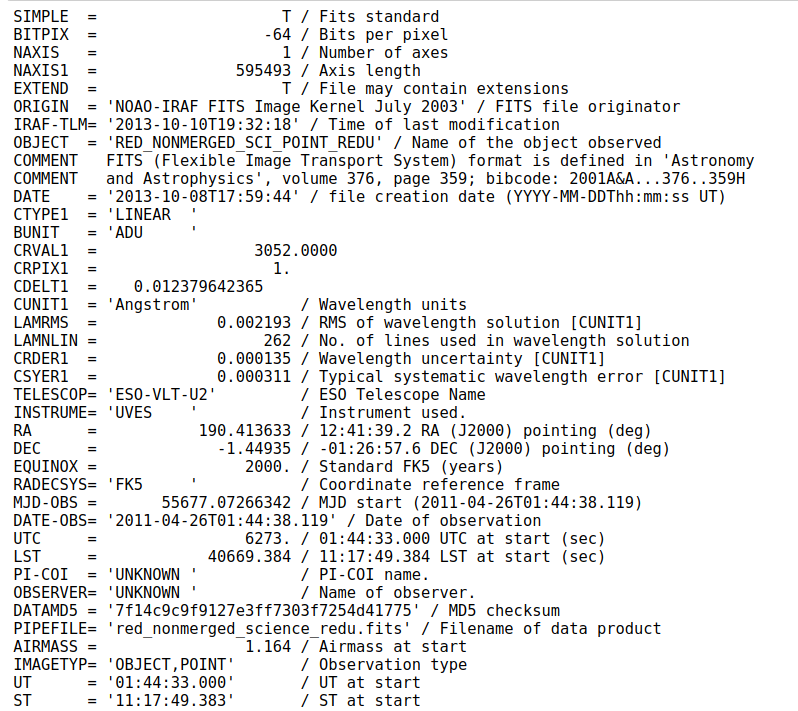
\includegraphics[width=10cm]{figuras/fits_header.png}
\caption{O trecho do cabeçalho do arquivo FITS da estrela }
\label{fig:fits-header}
\end{figure}

O componente em sequência do cabeçalho, quando presente, possui um vetor que pode ter desde 1 a 999 dimensões. Esta seção representa o dado astronômico capturado, como os valores do fluxo de um espectro estelar ou uma imagem de um objeto celeste. Os dados podem ter um de 5 possíveis tipos de dados \citep{pence2010definition}:

\begin{enumerate}
    \item Inteiros de 8 bits
    \item Inteiros de 16 bits
    \item Inteiros de 32 bits
    \item Números reais de ponto flutuante de 32 bits
    \item Números reais de ponto flutuante de 64 bits
\end{enumerate}

Nesta seção será descrito o processo de conhecimento e ambientação com os dados astronômicos fornecidos e seu formato. Alguns conjuntos de dados fornecidos para isto são de observações reais do nosso Sol, da estrela Arcturus, de um referencial telúrico para ambas e de estrelas capturadas pelo espectrógrafo UVES \footnote{\url{https://www.eso.org/sci/facilities/paranal/instruments/uves.html}} \citep{2000SPIE.4008..534D}, que também faz parte do \textit{Very Large Telescope Array} \footnote{\url{https://www.eso.org/public/brazil/teles-instr/paranal-observatory/vlt/?lang}}. 

Para leitura e manipulação de dados no formato FITS foi usada a biblioteca \textit{Astropy}\footnote{\url{http://www.astropy.org}}, que é amplamente usado para processar computacionalmente diversos dados astronômicos \citep{astropy:2018}. 

Com a combinação dos dados fornecidos e o ferramental correto, foi possível abrir, analisar e visualizar o espectro de diversas estrelas. Dois exemplos de estrelas e seus espectros observados estão nas figuras \ref{fig:hd110379} e \ref{fig:sun}, que representam, respectivamente, a estrela HD110379 e o Sol. 

\begin{figure}[!tbp]
  \centering
  \subfloat[HD110379]{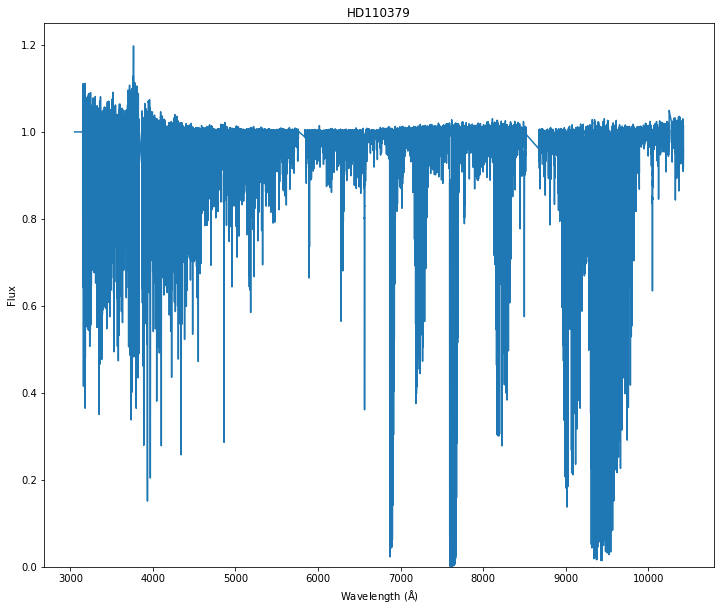
\includegraphics[width=0.5\textwidth]{figuras/hd110379_spectrum.png}\label{fig:hd110379}}
  \hfill
  \subfloat[Sol]{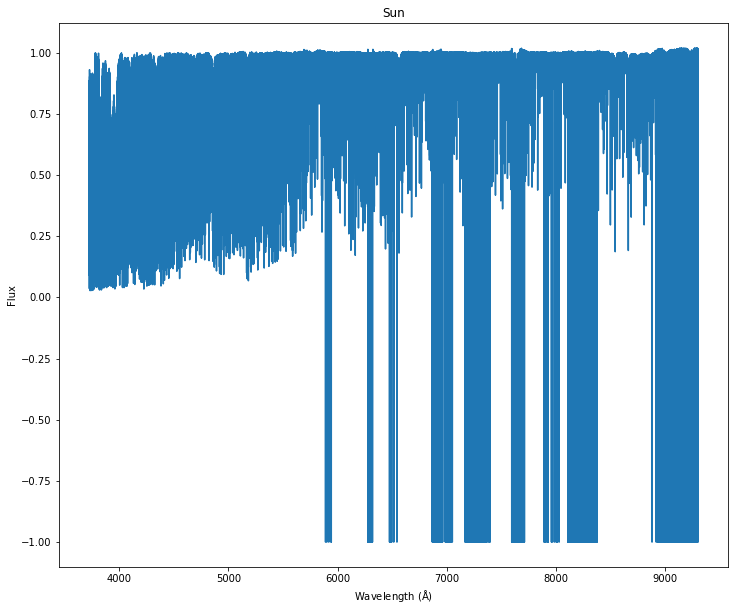
\includegraphics[width=0.5\textwidth]{figuras/sun_spectrum.png}\label{fig:sun}}
  \caption{Espectros observados de estrelas}
  \label{fig:two-stars}
\end{figure}

(falar mais sobre os espectros e suas diferenças, cada estrela tem um formato, fonte e normalização diferente)

\section{Divisão do sinal estelar pelo telúrico}

\section{DTW no sinal estelar}

\section{DTW no sinal atmosférico}